\documentclass[letter]{article}

%% Language and font encodings
\usepackage[english]{babel}
\usepackage[utf8x]{inputenc}
\usepackage[T1]{fontenc}
\usepackage{listings}
\usepackage{stmaryrd}
\usepackage{pgfplots}

%% Sets page size and margins
\usepackage[top=2cm,bottom=2cm,left=3cm,right=3cm,marginparwidth=1.75cm]{geometry}

%% Useful packages
\usepackage{amsmath}
\usepackage{amsfonts}
\usepackage{amssymb}
\usepackage{amsthm}
\usepackage{graphicx}
\usepackage[colorinlistoftodos]{todonotes}
%\usepackage[colorlinks=true, allcolors=blue]{hyperref}
\usepackage{array}
\usepackage[shortlabels]{enumitem}
\usepackage[final]{pdfpages}
\usepackage[normalem]{ulem}
\usepackage{cancel}
\usepackage{xspace,mdwlist}
\usepackage{algorithmic}
\usepackage{mathtools}
\usetikzlibrary{calc}

\usepackage{courier} %% Sets font for listing as Courier.
\usepackage{listings, xcolor}
\lstset{
tabsize = 4, %% set tab space width
showstringspaces = false, %% prevent space marking in strings, string is defined as the text that is generally printed directly to the console
numbers = left, %% display line numbers on the left
commentstyle = \color{green}, %% set comment color
keywordstyle = \color{blue}, %% set keyword color
stringstyle = \color{red}, %% set string color
rulecolor = \color{black}, %% set frame color to avoid being affected by text color
basicstyle = \small \ttfamily , %% set listing font and size
breaklines = true, %% enable line breaking
numberstyle = \tiny,
}



\DeclarePairedDelimiter{\ceil}{\lceil}{\rceil}
\DeclarePairedDelimiter{\floor}{\lfloor}{\rfloor}

\newtheorem{theorem}{Theorem}[section]
\newtheorem*{claim}{Claim}
\DeclareMathOperator*{\argmin}{\arg\!\min}

\def\coursename{CS 201: Data Structures}

%% make title box
\newcommand{\header}[1]{%
	\begin{center}
		\fbox{
			\begin{minipage}{6in}
				\textbf{\coursename} \hfill       \\
				\textit{#1} \hfill \textit{\today}
			\end{minipage}
		}
	\end{center}
	\vspace*{4mm}
}

\def\problem#1#2#3{
\fbox{
\begin{minipage}{0.8\textwidth}
{\sc #1:}

\begin{description*}
\item[Given:] #2
\item[Find:] #3
\end{description*}
\end{minipage}
}
\bigskip
}


\begin{document}

\header{Week 6: Sorting and recursion}

\begin{enumerate}[1.] 
    \item Give two concrete examples where insertion sort might be more suitable than selection sort\\



    \item fill in the blanks:\\

    
\begin{tabular}{|l|l|l|l|l|}
\hline
\begin{tabular}[c]{@{}l@{}}Sorting \\ algorithm\end{tabular} & \begin{tabular}[c]{@{}l@{}}Space\\  complexity\end{tabular} & Runtime & \#Swaps & \#Comparisons \\ \hline
Selection Sort &  & \begin{tabular}[c]{@{}l@{}}Worst:       \\ Best:\end{tabular} & \begin{tabular}[c]{@{}l@{}}Worst:       \\ Best:\end{tabular} & \begin{tabular}[c]{@{}l@{}}Worst: \\ Best:\end{tabular} \\ \hline
Insertion sort &  & \begin{tabular}[c]{@{}l@{}}Worst: \\ Best:\end{tabular} & \begin{tabular}[c]{@{}l@{}}Worst:\\ Best:\end{tabular} & \begin{tabular}[c]{@{}l@{}}Worst: \\ Best:\end{tabular} \\ \hline
Bubble sort &  & \begin{tabular}[c]{@{}l@{}}Worst: \\ Best:\end{tabular} & \begin{tabular}[c]{@{}l@{}}Worst: \\ Best:\end{tabular} & \begin{tabular}[c]{@{}l@{}}Worst: \\ Best:\end{tabular} \\ \hline
\end{tabular}

    \item Provide a brief outline for how quickSort in-place works. Include steps for partitioning.\\

    Quicksort:\\\\\\\\

    


    Partition:\\\\\\\\

    


    \newpage

    \item Oh no! The evil code mangler has rearranged all the code lines for quickSort in-place. You must put all the lines back in order to restore peace and unity!!!\\

    \begin{lstlisting}[language = Java , frame = trBL , firstnumber = 0 , escapeinside={(*@}{@*)}]
public static <E extends Comparable<E>> void quickSort(E[] array, int start, int stop) {
    
    int pivotIndex = partition(array, start, stop);  
    }
    if (start < stop) {
    quickSort(array, start, pivotIndex - 1);
    quickSort(array, pivotIndex + 1, stop);

private static <T extends Comparable<T>> int partition(E[] array, start, stop) {
    

    
    swap(array, start, pivotI);

    int pivotI = start;

    int up = start + 1;
    int down = stop;
    boolean done = false;

    E pivot = array[start];

    while (!done) {
        up++;
        down--;
        while (up < stop && array[up].compareTo(pivot) < 0) {
        }
    
        

        if (up < down) {
            swap(array, up, down);
            up++;
            down--;
        } else {
            
        }
        while (down > start && array[down].compareTo(pivot) > 0) {
        }
        done = true;
        swap(array, start, down);
    }
    
    return down;
}
\end{lstlisting}

    
     \item Given the quickSort algorithm above, what would be an example of an input array that results in worst case runtime: \\


     \item In the quickSort algorithm above, the pivot is always the first element in the current array. Explain why choosing a pivot this way not ideal, and come up with two better ways:\\



    \item fill in the blanks: (from Koffman - Wolfgang)
    
        \begin{itemize}
            \item [1.] A recursive method has two cases: ........ and..........
            \item [2.] Each recursive call must lead to a situation that is ........ to the .........
        \end{itemize}

    \item Here is a recursive method that works on a singly linekd list:\\

\begin{lstlisting}[language = Java , frame = trBL , firstnumber = 0 , escapeinside={(*@}{@*)}]
public int mystery(Node<E> head) {
    if (head == null) {
        return 5;
    }
    else {
        return 2 * mystery(head.next);
    }
}
\end{lstlisting}

    Suppose I call this recursive method on a linked list with three elements: head->1->2->3->null. Complete the diagram below to indicate the return value for each call to this method. It might be easier to start with the 4th call and work your way back towards the 1st call.\\

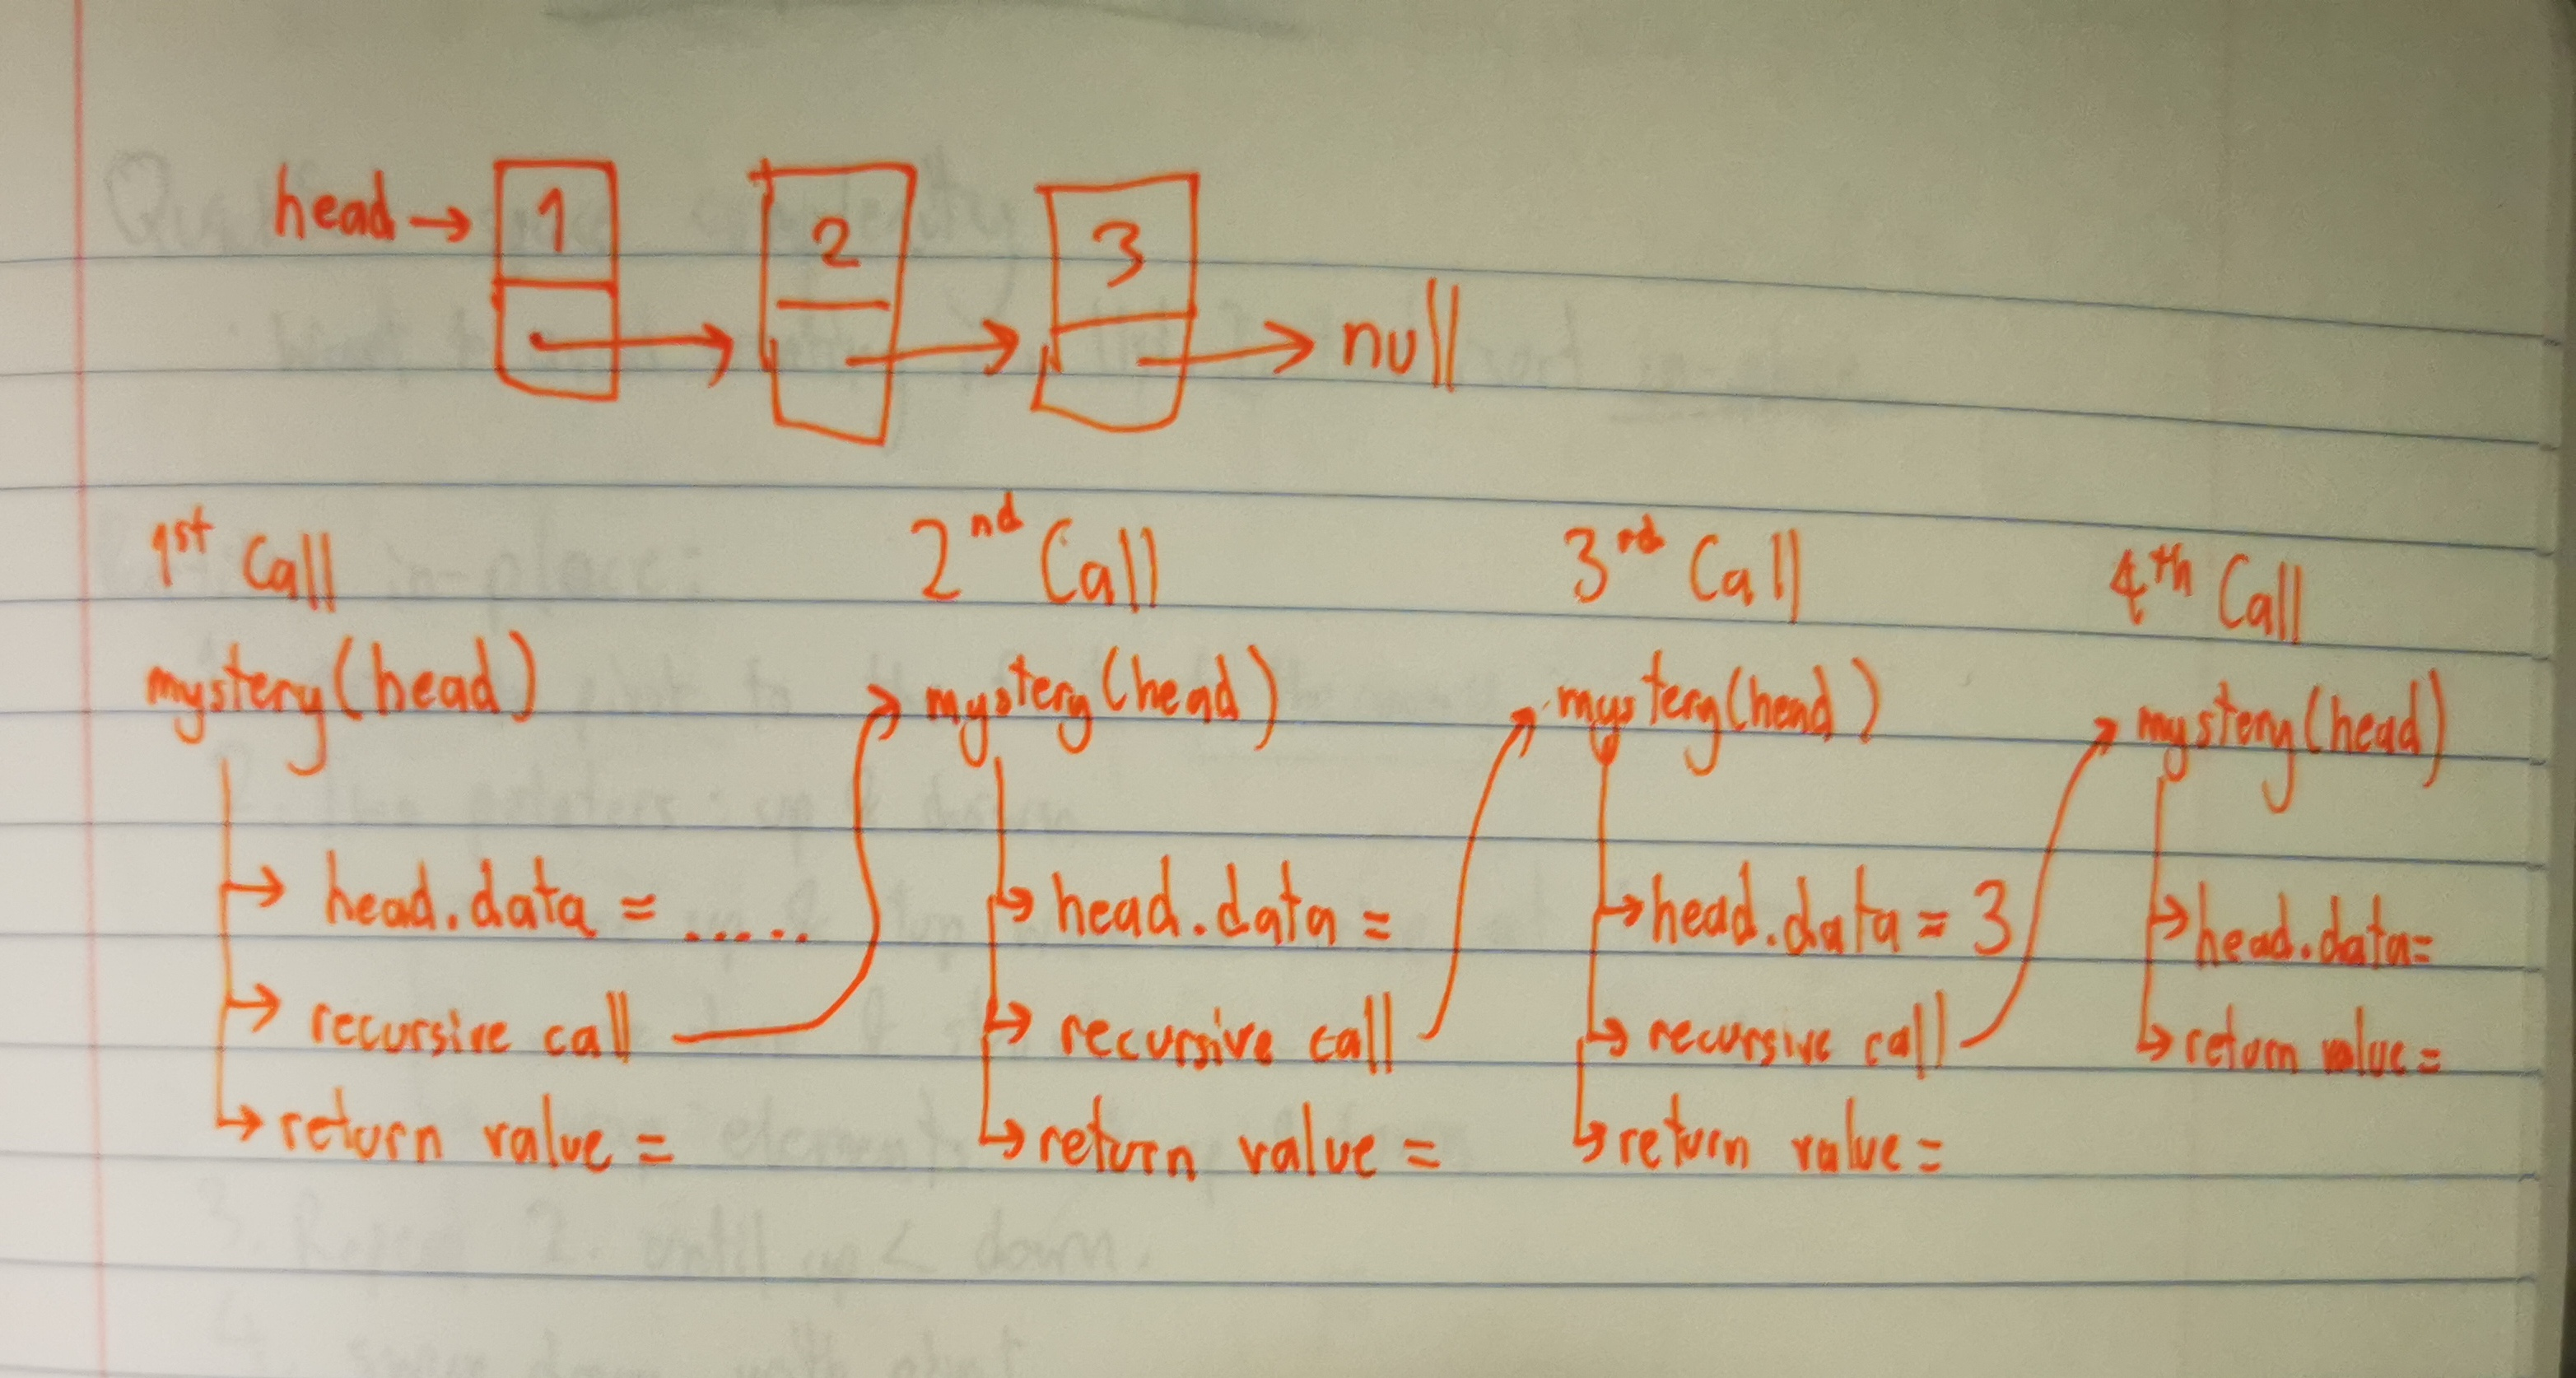
\includegraphics[scale = 0.10]{Question.jpg}\\


    \item Write a linked-list method public void replace(E oldItem, E newItem) that replaces all occurences of oldItem with newItem. You must use recursion. (hint: use helper methods).


\begin{lstlisting}[language = Java , frame = trBL , firstnumber = 0 , escapeinside={(*@}{@*)}]
public void replace(E oldItem, E newItem) {
    ...
}










...
\end{lstlisting}

    \item MergeSort is a sorting algorithm that performs the following:\\

    \begin{enumerate}
        \item Split the array into two halves
        \item Sort the left half
        \item Sort the right half
        \item Merge the two halves to form a sorted array
    \end{enumerate}

    Below is one implementation of mergeSort that works on an int[] array. Fill in the blanks to finish the implementation.
    \begin{lstlisting}[language = Java , frame = trBL , firstnumber = 0 , escapeinside={(*@}{@*)}]

//Combines two sorted array left and right into a single sorted array a.
public static void merge(int[] left, int[] right, int[] a) {
    //you can assume that this function works perfectly. 
}

public static void mergeSort(int[] a, int lo, int hi) {
    //If array size <= 1, then ...
    if (a.length <= 1) {
        
    }

    //Create two subarrays left and right
    int mid = lo + (hi-lo)/2;
    int[] left = new int[mid];
    int[] right = new int[a.length - mid];

    //Copy half of the array into left
    for (int i = 0; i < mid; i++) {
         
    }

    //Another half into right
    int k = 0;
    for (int j = mid; j < a.length; j++) {

        
    }
    //What else do we have to do? Hint: recursive case



    

}
    \end{lstlisting}

    \item Can you work out the big-O for mergeSort?\\

    

\end{enumerate}
\end{document}
